\section{METHODOLOGY}
\label{sec:methodology}

The main objective of this work was the creation of a base system for communication and exchange of information between autonomous agents through MAVLink protocol.
Agents must be able to share informations such as your current position, your current status (whether they are on a mission or not), what mission they are in, as well as having the ability to send missions to other agents.

The project was based on framework ROS (Robot Operating System), which provides a platform for research and development of robotic systems, possessing abstraction layers for communication, visualization and others.
As control platform, the autopilot ArduPilot had been used in two different kind vehicles, a land based (figure \ref{fig:rover}) and aerial (figure \ref{fig:quad}).
Both have global positioning sensor (GPS), altitude, and communication via radio, which can send and receive data from a base station.

\begin{figure}
        \centering
        \begin{subfigure}[b]{0.3\textwidth}
                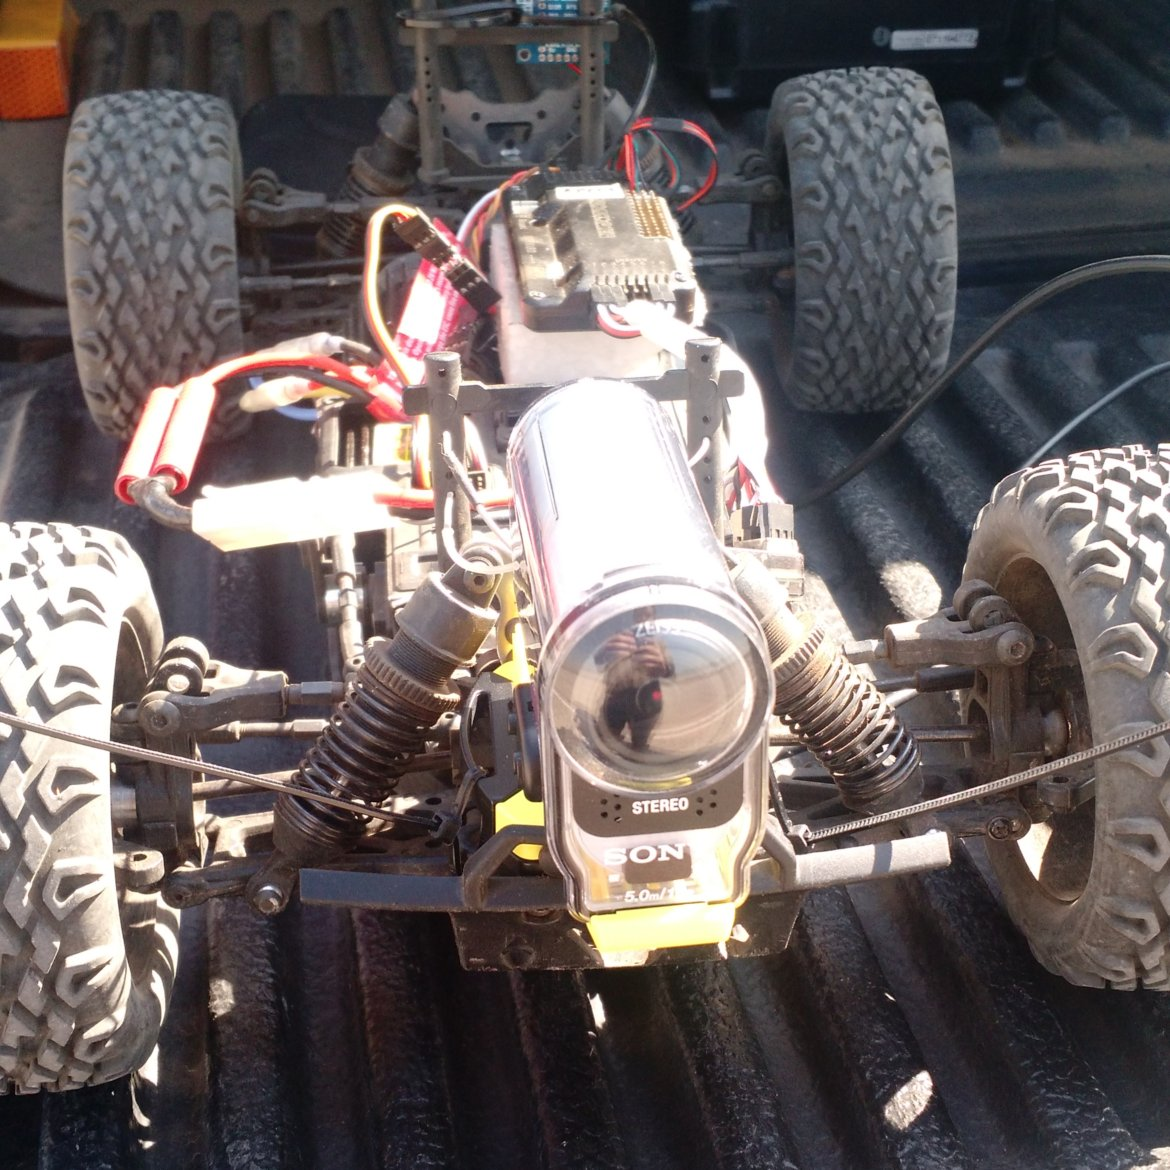
\includegraphics[width=\textwidth]{img/rover.jpg}
                \caption{Rover}
                \label{fig:rover}
        \end{subfigure}
        \quad
        \begin{subfigure}[b]{0.3\textwidth}
                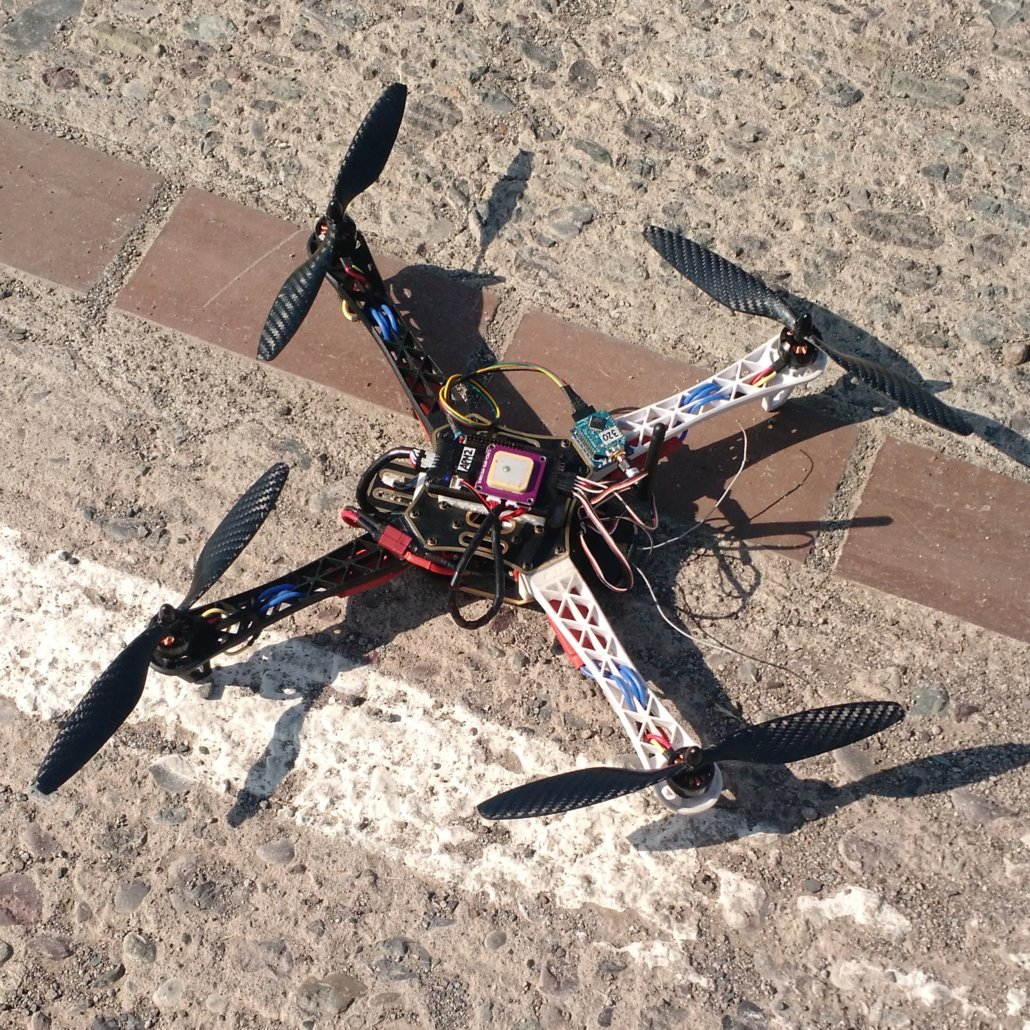
\includegraphics[width=\textwidth]{img/quad.jpg}
                \caption{Quadcopter}
                \label{fig:quad}
        \end{subfigure}
        \caption{Agents used on experiments}
        \label{fig:agents}
\end{figure}

\subsection{MAVLink Protocol} % (fold)
\label{sub:mavlink_protocol}

The MAVLink protocol was constructed to serve as common language between a ground control station and a autonomous robot.
It shows how to encode and decode data using a header-only message, describing a set of message types used to identify the message content.

A MAVLink message consists of a package with a minimum of 8 bytes and 263 bytes as maximum.
As can be seen in the figure \ref{fig:mavlink_message}, the package is divided into several slots, each one with a specific description.
The table \ref{table:mavlink_package} list and describe all slots of a MAVLink package.

\begin{figure}
  \centering
  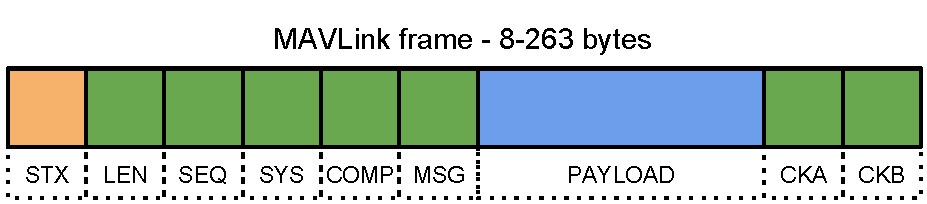
\includegraphics[width=0.9\columnwidth]{img/MAVLinkpackage.pdf}
  \caption{MAVLink Package description}
  \label{fig:mavlink_message}
\end{figure}

\begin{table}
    \begin{tabular}{|m{0.15\columnwidth}|m{0.75\columnwidth}|}
    \hline
    Slot    & Description                                                              \\ \hline
    STX     & Indicate a new package                                                   \\ \hline
    LEN     & Indicate the total length of the payload                                 \\ \hline
    SEQ     & Package sequence                                                         \\ \hline
    SYS     & ID of the sending MAV system                                             \\ \hline
    COMP    & ID of the sending component inside the MAV                               \\ \hline
    MSG     & ID of the message describing what type of message will be in the payload \\ \hline
    PAYLOAD & Data of the message                                                      \\ \hline
    CKA     & Checksum A (low byte)                                                    \\ \hline
    CKB     & Checksum B (high byte)                                                   \\ \hline
    \end{tabular}
    \caption {MAVLink Package slot description}
    \label{table:mavlink_package}
\end{table}

The protocol can handle various types of data, having support to fixed-size integer data, floats with single precision point, and array of these types.
The supported types are: \emph{char, uint8, int8, uint16, int16, uint32, int32, uint64, int64, float, double}.

The main objective of the protocol was the be fast and safety, but there are some drawbacks, as the need of extra bytes to track the messages, but it can detect the lost of packages and check the content.

% subsection mavlink_protocol (end)

\subsection{ROS Communication System} % (fold)
\label{sub:ros_communication_system}

The ROS environment was created aiming the decoupling between any part of the system, creating a system of communication that do not link directly two parts of the code.
To create this environment, two main concepts were created, the nodes and the topics.
Each node is a piece of code that executes a determined behavior, like control the velocity of the motors of a car or capture images from a camera.
Each topic is a address where the data is read and write by the nodes using the actions of subscribing and/or publishing to that topic.
This guarantee the possibility of the code run in different computers, like using a team of robots, each one with it individual computer for example.

The figure \ref{fig:ros_environment} show a representation of the ROS environment, where there are many nodes exchanging information using the topics. One important note about that type of communication is about the registration of the nodes and the initial meeting among then, that is made by the called \emph{master node}, that waits for the initialization of any node, and any request to publish or subscribe to one topic and make all the necessary connections.

\begin{figure}
  \centering
  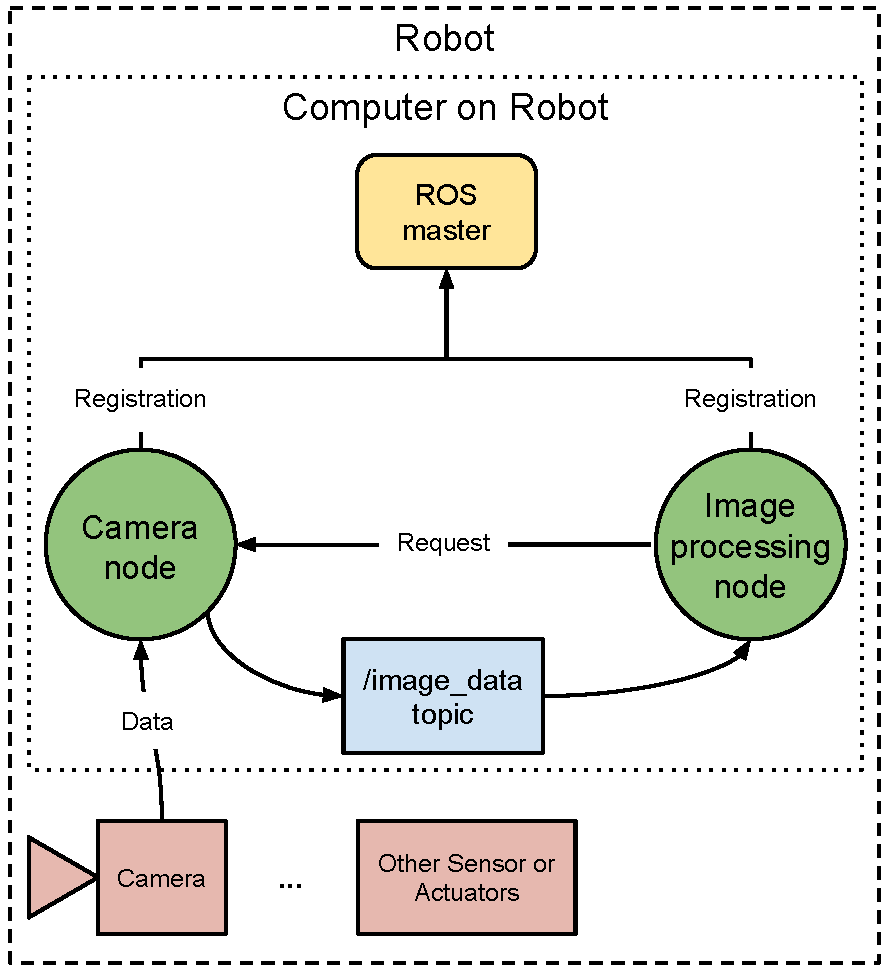
\includegraphics[width=0.9\columnwidth]{img/ros_environment.pdf}
  \caption{ROS Environment}
  \label{fig:ros_environment}
\end{figure}

% subsection ros_communication_system (end)

\subsection{Project Architecture} % (fold)
\label{sub:architecture}

In general, the architecture for controlling a robot using the ArduPilot platform is made by a base station which communicates with the agent via the MAVLink protocol, sending commands and tasks.
The onboard controller is responsible to receive and threat theses messages, making the necessary decisions to accomplish the sent objectives.
However, this strategy only guarantees the control of one agent at a time, and does not allow the exchange of information between an agent team.
The work developed here proposes an extension to this architecture in order to provide a communication and intelligence layer for agents, serving as basis for the development of more complex tasks that require the use of a set of robots.

Figure \ref{fig:architecture} shows the layout of the developed architecture, marking the addition in the context of communication in the pre-existing control layer.
The manner in which this strategy was set aims to promote transparency about the origin of the commands received by the agents, because similar to messages sent by the base station, the system developed also communicates through MAVLink commands, which makes interaction with agents direct and simple.

\begin{figure}
  \centering
  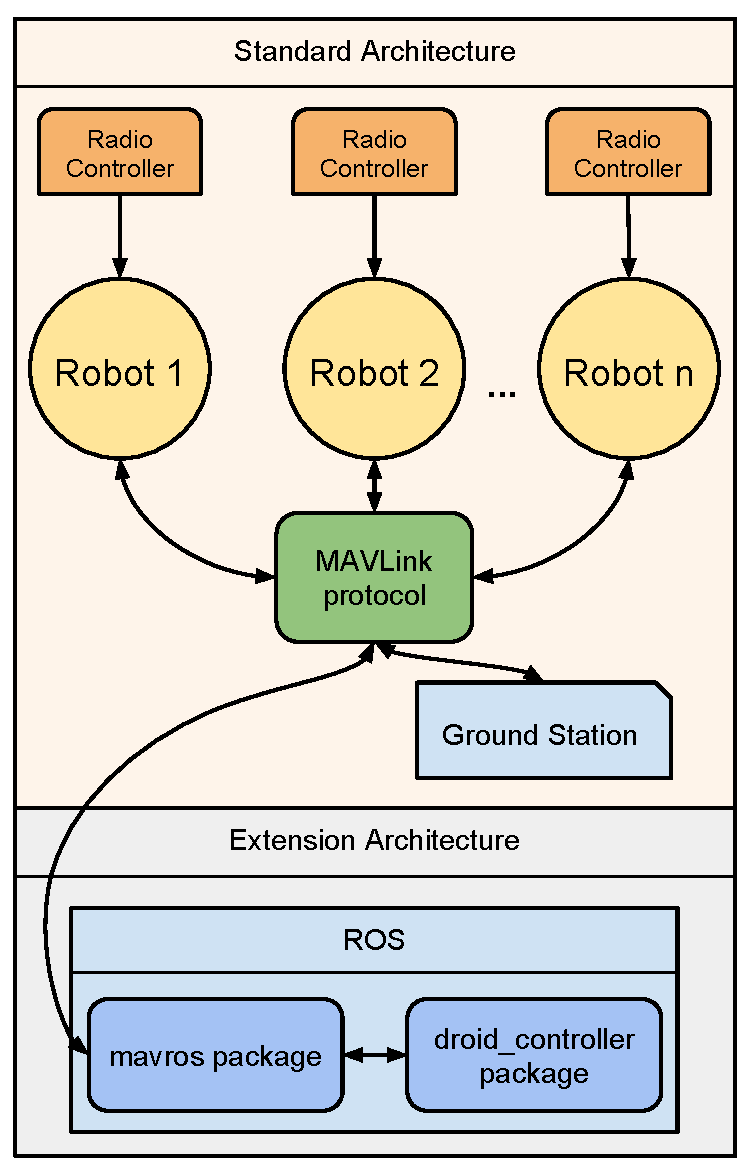
\includegraphics[width=0.8\columnwidth]{img/arquitetura.pdf}
  \caption{System Architecture}
  \label{fig:architecture}
\end{figure}

The MAVLink protocol is a standard regarding communication with autonomous systems, in this way there are several libraries that abstract the low-level details in communication, providing an interface for sending and receiving data transparently.
One of these libraries, implemented within the context of the ROS is the \emph{mavros} package.
This package continue in development by a group of nonprofit developers who created the tool because they see the opportunity of using these systems as autonomous intelligent agents.

The \emph{mavros} package is able to encode and decode messages in MAVLink, extract information and then format them into ROS messages, making the communication with a ArduPilot direct to the ROS infrastructure, providing easy access to other packages for these information.

Based on this structure, was created the package \emph{Droid Controller}, which contains a set of classes and algorithms that perform the reading of information from the agents and performs processing and exchange of information between them.

% subsection arquitetura (end)

\subsection{Droid Controller Package} % (fold)
\label{sub:droid_controller_package}

The \emph{Droid} package stacks over the \emph{mavros} package using it connection and MAVLink message handler.
The main goal was to create a set of classes that listen, store and share data from the agents and also create a interaction interface where is possible to request this data, send commands or missions.
This package should serve as basis for the creation of complex missions using the shared information between the robots.

The following are the main classes of the \emph{Droid} package:

\begin{description}
  \item[\textbf{Droid}] \hfill \\
    The Droid class is the base class to any specialized vehicle.
    It retains all important data about the robot like its current position, status of motors, MAVLink mode, current mission, battery status and others.
    Also export functions to get/set configuration parameters, send mission or arm the robot, among others.
  \item[\textbf{DroidCopter}] \hfill \\
    Specific class for a aerial robot, like a quadrotor.
    It uses and extends the Droid class, adding behaviors to return the craft to ground based on the level of remaining battery, and perform the initialization sequence for a mission.
  \item[\textbf{DroidRover}] \hfill \\
    Class that control a terrestrial robot, like a rover.
    Extends the Droid class to perceive for obstacles while a mission, requesting for another agent to continue the mission if it's not possible to complete it.
\end{description}

As a example of integration and exchange of information, the Droid class implements a follow behavior, where a agent is capable of maintain a certain distance from another based on its current global position and the position of another robot.
This behavior can be extended to create a squad behavior using various robots.

% subsection droid_controller_package (end)
